\documentclass[a4paper, 12pt, onepage]{article}
\usepackage[utf8]{inputenc}
\usepackage[russian]{babel}
\usepackage{fullpage}
\usepackage{indentfirst}
\usepackage{graphicx}
\usepackage{cmap}
\usepackage{amsmath}
\usepackage{amssymb}
%\usepackage{pdfpages}
\usepackage{tikz}

\usepackage[pdftex, unicode, pdfstartview=FitH, colorlinks, linkcolor=black, citecolor=blue, urlcolor=blue]{hyperref}
\usepackage{url}
\def\UrlFont{\rmfamily}

\usepackage{setspace}
\onehalfspacing

\usepackage{cyrtimes}
\renewcommand\ttdefault{cmtt}

\frenchspacing
\sloppy
\selectlanguage{russian}

\begin{document}

\author{Красильников Иван}
\title{}
\maketitle

\subsection*{Задача 1}
\textbf{1.} Вероятность, что пришедшее письмо является спамом:
\begin{align}
  P(S) &= \sum_{x_1, x_2, x_3, x_4, x_5} P(S | X_1=x_1, \ldots, X_5=x_5) P(X_1=x_1, \ldots, X_5=x_5) = \\
       &= \sum_{x_1, x_2, x_3, x_4, x_5} \prod_{i=1}^5 P(S | X_i=x_i) P(X_1=x_1, \ldots X_5=x_5),
\end{align}
где сумма берётся по всем 32 возможным значениями переменных $x_i$ (каждая переменная равна либо 0, либо 1).

\medskip

\textbf{2.} Из задания следует, что величины $X_2, X_3, X_5$ имеют следующее совместное распределение:

\medskip

\begin{tabular}{|c|c|c|c|}
  \hline
  $X_2$ & $X_3$ & $X_5$ & $P(X_2, X_3, X_5)$ \\
  \hline
  $1$ & $1$ & $1$ & ${1/2}$ \\
  $0$ & $1$ & $1$ & ${1/4}$ \\
  $0$ & $0$ & $1$ & ${1/8}$ \\
  $0$ & $0$ & $0$ & ${1/8}$ \\
  \hline
\end{tabular}

\medskip

Предполагая, что $X_1$ и $X_4$ независимы друг от друга и от $X_2, X_3, X_4$, сумму в уравнении (1) можно раскрыть так:

\begin{align*}
  P(S) = \sum_{x_4=0}^1 \sum_{x_5=0}^1 P(S|X_4=x_4) & P(S|X_5=x_5) P(X_4=x_4) P(X_5=x_5) \cdot (  \\
    & \frac{1}{2} P(S | X_2=1) P(S | X_3=1) P(S | X_5=1))\ + \\
    & \frac{1}{4} P(S | X_2=0) P(S | X_3=1) P(S | X_5=1))\ + \\
    & \frac{1}{8} P(S | X_2=0) P(S | X_3=0) P(S | X_5=1))\ + \\
    & \frac{1}{8} P(S | X_2=0) P(S | X_3=0) P(S | X_5=0)))
\end{align*}

\subsection*{Задача 3}
Я реализовал задачу с использованием python, 
{
\footnotesize
\begin{verbatim}
#!/usr/bin/env python
# coding: utf8
from numpy import *
import matplotlib.pyplot as pyplot
import sys, math, random

def delta(val):
    if abs(val) < 1e-9:
        return 1
    else:
        return 0

# функция ковариации из задания
def R_eps(x, y, eps):
    N = len(x)
    dist2 = sum((x[i] - y[i])**2 for i in range(N))
    return (1 - eps) * math.exp(-0.3 * dist2) + eps * delta(dist2)

# считает матрицу ковариации для набора точек
def CovarianceMatrix(points, cov_func):
    N = len(points)
    res = matrix(zeros((N, N)))
    for i in range(N):
        for j in range(N):
            res[i, j] = cov_func(points[i], points[j])
    return res

# генерация многомерной нормальной с нулевым средним
def MultivariateNormal(cov_matrix):
    N = cov_matrix.shape[0]
    L = linalg.cholesky(cov_matrix)  # cov_matrix = L * L^T
    X = matrix(zeros((N, 1)))        # вектор со стандартными нормальными
    for i in range(N):
        X[i, 0] = random.normalvariate(0, 1)
    return L * X

# генерация случайной реализации поля в заданном наборе точек
def GenerateField(points, cov_func):
    R = CovarianceMatrix(points, cov_func)
    return MultivariateNormal(R)

# Предсказание значения поля в новой точке методом кригинга.
# R, u - матрица ковариации и значения поля для точек обучающей выборки
# r - вектор ковариаций точек обучающей выборки с новой точкой.
def Kriging(R, u, r):
    Rinv = linalg.inv(R)
    a = r.transpose() * Rinv       # a = r^T R^{-1}
    return a * u


X = [[-1,-1,0], [-1,0,0], [-1,1,0], [0,-1,0], [0,0,0], [0,1,0], [1,-1,0], [1,0,0], [1,1,0],
     [-1,-1,1], [-1,0,1], [-1,1,1], [0,-1,1], [0,0,1], [0,1,1], [1,-1,1], [1,0,1], [1,1,1]]
assert len(X) == 18

random.seed(13058)
fig = pyplot.figure()
fig_plot = fig.add_subplot(111)
pyplot.xlabel('eps')
pyplot.ylabel('F(eps)')

for inst in range(5):
    U = GenerateField(X, lambda x, y: R_eps(x, y, 0.1))

    plot_x = []
    plot_y = []

    for i in range(100):
        eps = i / 100.0;
        R = CovarianceMatrix(X, lambda x, y: R_eps(x, y, eps))

        U2 = zeros((9, 1))
        Ueps = zeros((9, 1))
        for i in range(9, 18):
            U2[i - 9] = U[i]
            Ueps[i - 9] = Kriging(R[0:9, 0:9], U[0:9], R[0:9, i])

        F = sum((U2[i] - Ueps[i])**2 for i in range(9))

        plot_x.append(eps)
        plot_y.append(F)

    fig_plot.plot(plot_x, plot_y)

fig.savefig('figure.pdf')
\end{verbatim}
}

\newpage
График $F(\varepsilon)$ для пяти случайных реализаций поля:
\begin{figure}[htp]
  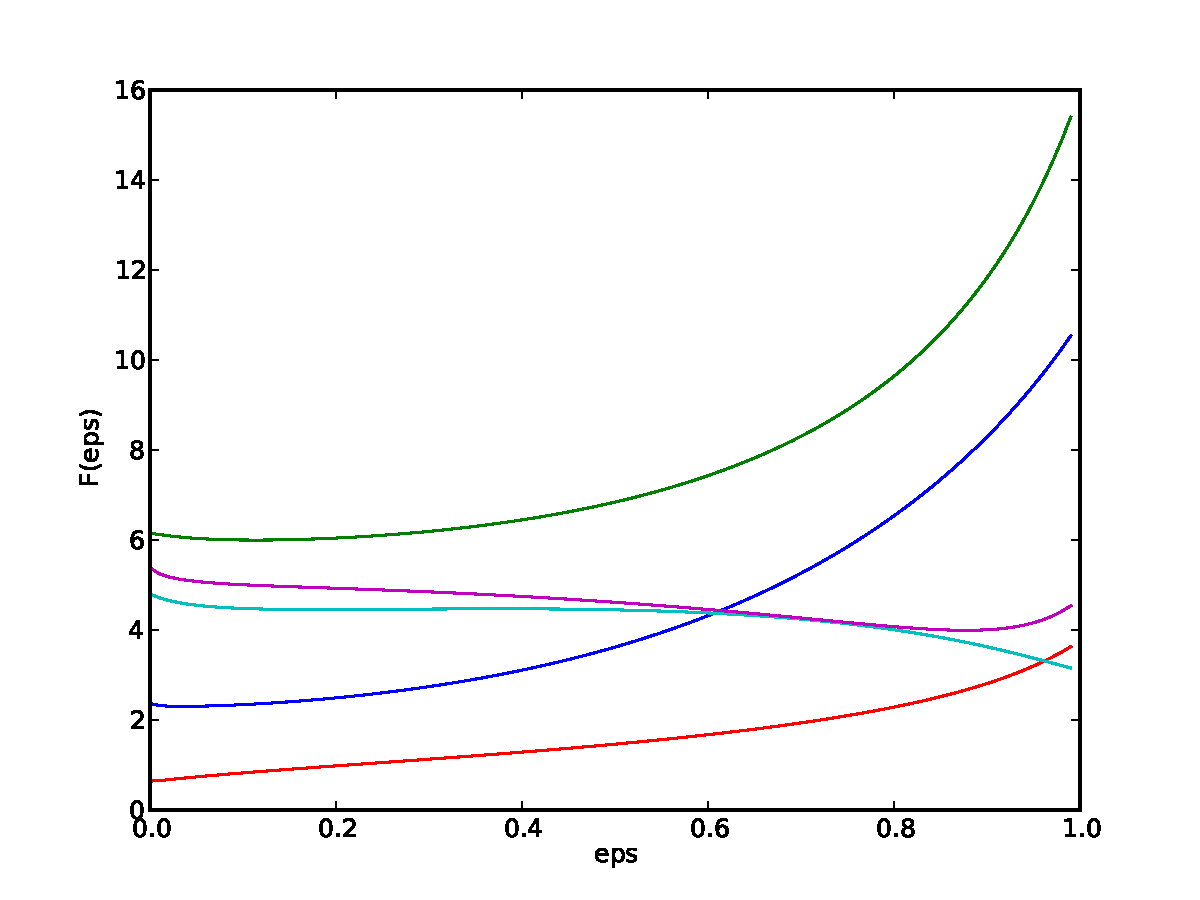
\includegraphics[scale=0.5]{figure.pdf}
\end{figure}

График $F(\varepsilon)$ для еще 10 других случайных реализаций поля:
\begin{figure}[htp]
  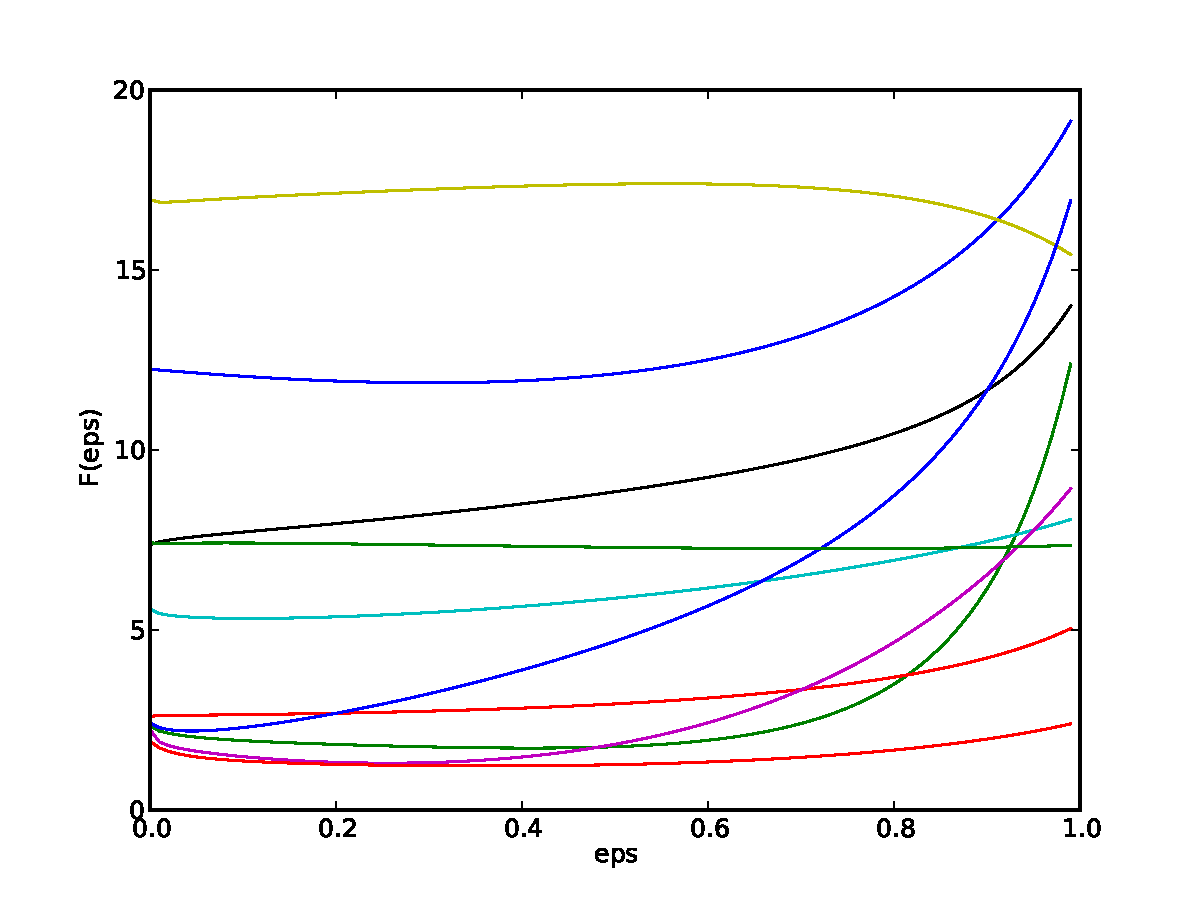
\includegraphics[scale=0.5]{figure2.pdf}
\end{figure}

Можно заметить, что у многих реализаций минимальное значение достигает в левой части графика,
при значениях, близких к $\varepsilon = 0.1$, при котором генерировалось поле,
и причем рядом с этим значением существуют большие интервалы, в которых $F(\varepsilon)$
мало меняется. Таким образом можно заключить, что метод кригинга достаточно устойчив
к выбору $\varepsilon$.

На некоторых графиках это не так, и минимум достагается далеко от $\varepsilon=0.1$,
что можно объяснить малым объемом выборки (всего 9 наблюдений) и большой долей
случайности в данных.

\end{document}
